\documentclass[a4paper,12pt]{article}
\usepackage[preprint]{neurips_2024}
\usepackage[a4paper,margin=1in]{geometry}
\usepackage[T1]{fontenc}
\usepackage[utf8]{inputenc}
\usepackage{microtype}
\usepackage{graphicx}
\usepackage{booktabs}
\usepackage{amsmath,amssymb}
\usepackage{multirow}
\usepackage{array}
\usepackage{float}
\usepackage{caption}
\usepackage{subcaption}
\usepackage{xcolor}
\usepackage{pgfplots}
\usepackage{titlesec}
\usepackage{tocloft}
\usepackage{url}
\usepackage[numbers,sort&compress]{natbib}
\usepackage[colorlinks=true, linkcolor=blue, citecolor=blue, urlcolor=blue]{hyperref}
\makeatletter
\renewcommand{\@noticestring}{}
\makeatother

\pgfplotsset{compat=1.18}
\bibliographystyle{IEEEtran}
\setlength{\cftbeforesecskip}{1pt}
\setlength{\cftbeforesubsecskip}{0pt}
\renewcommand{\cftsecfont}{\small}
\renewcommand{\cftsubsecfont}{\small}
\renewcommand{\cftsecpagefont}{\small}
\renewcommand{\cftsubsecpagefont}{\small}
\setlength{\textfloatsep}{10pt plus 2pt minus 2pt}
\setlength{\floatsep}{8pt plus 2pt minus 2pt}
\setlength{\intextsep}{8pt plus 2pt minus 2pt}
\setlength{\abovecaptionskip}{4pt}
\setlength{\belowcaptionskip}{2pt}

\title{ArxivRAG: Design and Optimization of a Retrieval-Augmented Generation System for arXiv Papers}

\author{
Raymond Denis Vladu \\
Student ID: K12306746 \\
Institute of Machine Learning, JKU Linz
}

\date{May 2026}

\begin{document}
\maketitle
\tableofcontents

\newpage

\section{Introduction}

This report documents the practical design, implementation, and optimization of \textit{ArxivRAG}, a Retrieval-Augmented Generation system specialized for querying arXiv papers. Retrieval-Augmented Generation combines external retrieval systems with language models to improve factual grounding and access to domain-specific knowledge \cite{lewis2020rag}. The focus in this report is not on general RAG theory, but on the engineering decisions required to build a working scientific retrieval system and evaluate it under controlled conditions. Although the system architecture section includes the operational ArxivRAG pipeline for context, the primary focus of this report is the experimental benchmarking pipeline used to compare retrieval configurations.

The central challenge in this project was retrieval quality. In scientific document collections, relevant evidence may be buried inside long PDFs, mathematical sections, appendices, or fragmented methodology descriptions. Therefore, system performance depends heavily on how papers are parsed, chunked, and ranked before generation occurs.

To investigate this systematically, a reproducible benchmark environment was created using a frozen corpus snapshot and a small, manually authored evaluation dataset. Two experimental phases were conducted:

\begin{itemize}
    \item comparison of four chunking strategies,
    \item parameter sweeps over retrieval mode, top-k values, and reranking.
\end{itemize}

The objective was to determine which configuration provides the strongest practical retrieval performance for the deployment of ArxivRAG.

\textbf{Important Note:} All experiments in this report are retrieval-only. Configuration choices (chunking strategy, top-$k$, dense vs.\ hybrid retrieval, and reranking) are selected using Recall@k, Precision@k, and MRR only, without evaluating generated answers or any LLM output quality.

\section{System Architecture}

ArxivRAG was implemented as a modular retrieval-generation stack with explicit separation between corpus management, vector indexing, retrieval orchestration, and answer synthesis. The implementation follows a ``retrieve-then-read'' design, where retrieval quality is optimized independently before downstream generation.

\subsection{Infrastructure}

The evaluation stack was containerized with Docker Compose to keep storage and indexing dependencies reproducible across runs. The following service images were used:

\begin{itemize}
    \item \textbf{minio/minio}: object storage for downloaded PDFs, processed corpora and frozen benchmark snapshots.
    \item \textbf{qdrant/qdrant}: vector database for embeddings, metadata and similarity search.
\end{itemize}

Embeddings were generated with \texttt{google/embeddinggemma-300m}. The embedding model is based on the Gemma model family introduced by Google \cite{gemmateam2024gemma}. Optional reranking used \texttt{cross-encoder/ms-marco-MiniLM-L-6-v2}. This component split enabled independent control of indexing, retrieval, and generation settings during experiments.

\newpage

\subsection{Operational ArxivRAG Pipeline}

The following sequence describes the production retrieval-generation workflow of the running ArxivRAG system:

\begin{enumerate}
    \item arXiv search using topic keywords,
    \item paper download in PDF format,
    \item PDF text extraction,
    \item structural parsing into sections,
    \item chunk generation,
    \item embedding creation,
    \item indexing into Qdrant,
    \item dense or hybrid retrieval,
    \item optional reranking,
    \item downstream answer generation.
\end{enumerate}

Operationally, retrieval is executed over chunk embeddings stored in Qdrant, with two retrieval modes: dense cosine retrieval and hybrid retrieval (dense + BM25 score fusion, weighted 0.5/0.5 after min-max normalization)\cite{robertson2009bm25}. The dense path supports Maximal Marginal Relevance (MMR, $\lambda=0.7$) for diversity-aware selection, and an optional cross-encoder reranking stage can reorder a candidate pool before selecting final top-$k$ chunks\cite{carbonell1998mmr}\cite{nogueira2019bert}.

For generation, ArxivRAG uses DeepSeek through an OpenAI-compatible client (\texttt{model=deepseek-chat}) with default decoding parameters \texttt{temperature=0.7}, \texttt{max\_tokens=2048}, and a configured context limit of 8192 tokens. DeepSeek-V3 is a Mixture-of-Experts large language model designed for efficient large-scale training and inference \cite{deepseek2024v3}. Retrieved context is budgeted heuristically before prompting (token-aware character allocation per chunk, truncation when needed, and retry with fewer chunks if context length is exceeded).

\subsection{Prompt Engineering}

Prompt design was intentionally constrained to reduce stylistic hedging and enforce grounded, technical answers. The system message instructs the model to:

\begin{itemize}
    \item answer directly and authoritatively,
    \item avoid phrases such as ``Based on the provided context'',
    \item use markdown structure for readability,
    \item include technical entities (model names, architectures, methodologies) when present in evidence,
    \item rely only on supplied retrieved context.
\end{itemize}

The user prompt then injects retrieved passages with explicit source metadata (paper title, arXiv identifier, section label), followed by the question. This two-part prompt template was used to improve factual grounding while keeping generation behavior consistent across retrieval configurations.

\newpage

\section{Evaluation Dataset and Reproducibility}

A manually created benchmark dataset of 49 evaluation examples was constructed. Each evaluation example was represented as a structured record with four fields:

\begin{itemize}
    \item unique identifier,
    \item topic keywords,
    \item natural language question,
    \item manually curated gold passages.
\end{itemize}

This structure was chosen to separate retrieval intent, retrieval input, and relevance supervision:

\begin{itemize}
    \item \textbf{ID} provides a stable key for logging, metric aggregation, and reproducible reruns.
    \item \textbf{Topic keywords} define corpus-freezing scope (paper discovery) independent of wording in the final question.
    \item \textbf{Question} captures realistic user intent for retrieval evaluation.
    \item \textbf{Gold passages} provide passage-level relevance anchors used by Recall@k, Precision@k, and MRR scoring.
\end{itemize}

The separation between topic keywords and question text is intentional: in practical use, paper collection is often driven by broad domain terms, while evaluation queries are narrower and phrased naturally. Keeping these fields distinct reduces leakage between corpus construction and retrieval scoring, and makes experiments easier to reproduce and audit.

\begin{table}[htbp]
\centering
\caption{Example structure of evaluation records (illustrative subset).}
\small
\setlength{\tabcolsep}{4pt}
\begin{tabular}{p{1.7cm}p{2.6cm}p{4.8cm}p{5.0cm}}
\toprule
ID & Topic keywords & Question & Gold passages (summary) \\
\midrule
\texttt{ev\_001} & transformer, scaling laws & What evidence is reported about loss scaling with model size? & Kaplan et al.\ scaling-law section; reported power-law fit and regime assumptions. \\
\texttt{ev\_014} & retrieval augmented generation, dense retrieval & Which component is responsible for first-stage candidate retrieval in RAG? & Retriever stage description; dense encoder + nearest-neighbor index role. \\
\texttt{ev\_032} & diffusion models, image generation & How is classifier-free guidance defined and where is it applied? & Guidance formulation in sampling equations; conditional/unconditional score interpolation. \\
\bottomrule
\end{tabular}
\end{table}

Because live arXiv search results may change over time, reproducibility required freezing the corpus used during evaluation. For each benchmark topic:

\begin{enumerate}
    \item arXiv was queried using topic keywords,
    \item candidate papers were ranked by abstract relevance,
    \item top papers were downloaded,
    \item PDFs were stored in MinIO,
    \item a manifest mapped benchmark queries to their evaluation corpus.
\end{enumerate}

This ensured later experiments used identical documents independent of future arXiv updates.

\newpage

\section{Methodology}

\subsection{Experimental Pipeline Overview}

In addition to the operational ArxivRAG pipeline, this work uses a separate experimental pipeline to evaluate retrieval quality in a controlled and reproducible way. The evaluation workflow consists of:

\begin{enumerate}
    \item define evaluation queries with manually authored gold passages,
    \item freeze the document corpus per query topic using a manifest,
    \item select one chunking strategy and re-index the same frozen corpus,
    \item run retrieval-only evaluation on the full query set,
    \item compute Recall@k, Precision@k, and MRR for that run,
    \item repeat Step 3--5 for all chunking strategies (Phase 1),
    \item select the best chunker, then sweep retrieval settings (Phase 2),
    \item produce a report that presents all retrieval results, compares Phase 2 configurations, and states the final deployment recommendation.
\end{enumerate}


\subsection{Metrics}

Three standard information retrieval metrics were used\cite{manning2008ir}:

\begin{itemize}
    \item \textbf{Recall@k}: paper-level coverage in top-$k$, computed as
    \[
    \frac{|\text{retrieved paper IDs}_{k} \cap \text{gold paper IDs}|}{|\text{gold paper IDs}|}.
    \]
    \item \textbf{Precision@k}: proportion of top-$k$ chunks marked relevant.
    \item \textbf{MRR}: reciprocal rank of the first relevant chunk in the ranked list.
\end{itemize}

Chunk relevance for Precision@k and MRR used a hybrid rule: a chunk is relevant if either (i) its paper ID matches a gold document, or (ii) its embedding has cosine similarity $\geq 0.8$ to at least one manually authored gold passage. This thresholded passage criterion was used to score partial-document evidence when exact paper matches were insufficiently granular.

\subsection{Chunking Strategies}

Four chunking methods were implemented and compared:

\begin{enumerate}
    \item \textbf{Structure-Aware Overlap}: hierarchy-aware chunking over parsed sections/subsections, target 650 tokens, maximum 900 tokens, with overlap ratio 0.12 (approximately 78-token carryover from the previous chunk); abstract and conclusion blocks are preserved as standalone chunks.
    \item \textbf{Semantic Paragraph Grouping}: paragraph-level grouping via adjacent embedding similarity (threshold 0.75), with chunk cap at 900 tokens; falls back to structure-aware behavior if embeddings are unavailable.
    \item \textbf{Fixed Window Overlap}: sliding windows of 700 tokens with 150-token overlap (step size 550 tokens). Overlap units are \textit{tokens}, not characters or sentences.
    \item \textbf{Section-Level Chunking}: one chunk per subsection/section block, split only when block size exceeds 1500 tokens (midpoint paragraph split).
\end{enumerate}

All strategies were evaluated with abstract skipping enabled during indexing (\texttt{skip\_abstract=True}) to reduce shortcut retrieval from high-level summaries and force evidence retrieval from body content. Reference sections were removed for fixed-window chunking.

\subsection{Two-Phase Experimental Design}

\textbf{Phase 1 (Chunker Selection):} Determine the strongest chunking strategy under fixed retrieval settings. For each strategy, the same frozen paper set was re-indexed from scratch, then evaluated with:
\begin{itemize}
    \item dense retrieval only,
    \item top-$k=8$ (fixed),
    \item reranking disabled,
    \item MMR enabled by default (unless explicitly disabled),
    \item identical query set and frozen corpus manifest.
\end{itemize}

The Phase 1 winner was selected lexicographically by \texttt{Recall@k}, then \texttt{MRR}, then \texttt{Precision@k} to prioritize evidence coverage while preserving ranking quality.

\textbf{Phase 2 (Retrieval Configuration Sweep):} Using only the Phase 1 winning chunker, evaluate the Cartesian product of retrieval settings:

\[
top\text{-}k \in \{3,5,10\}
\]

\[
retrieval \in \{dense, hybrid\}
\]

\[
reranking \in \{false,true\}
\]

This yields 12 configurations in total (3 top-$k$ values $\times$ 2 retrieval types $\times$ 2 reranking states). Unlike Phase 1, which isolates chunking effects, Phase 2 isolates ranking-time effects while keeping corpus, chunking strategy, and evaluation set fixed. This two-step design reduces confounding between segmentation quality and retrieval/reranking hyperparameters.

\newpage

\section{Results}

\subsection{Phase 1: Chunking Comparison}

\begin{table}[htbp]
\centering
\caption{Phase 1 retrieval results.}
\begin{tabular}{lccc}
\toprule
Strategy & Recall@8 & Precision@8 & MRR \\
\midrule
Structure-Aware Overlap & 0.8776 & 0.3061 & 0.6511 \\
Semantic Paragraph Grouping & 0.6531 & 0.1556 & 0.3546 \\
Fixed Window Overlap & \textbf{0.9388} & \textbf{0.4362} & \textbf{0.7475} \\
Section-Level Chunking & 0.9184 & 0.3444 & 0.5931 \\
\bottomrule
\end{tabular}
\end{table}

Fixed Window Overlap produced the strongest results across all three metrics. This indicates that consistent local windows currently provide the best balance between preserving context and maintaining retrieval specificity.

\subsection{Phase 2: Retrieval Configuration Sweep}

\begin{table}[htbp]
\centering
\caption{Exhaustive Phase 2 results across all 12 retrieval configurations.}
\small
\setlength{\tabcolsep}{5pt}
\begin{tabular}{ccclll}
\toprule
top-k & Retrieval & Rerank & Recall@k & Precision@k & MRR \\
\midrule
\multirow{4}{*}{3}  & Dense  & No  & \textbf{0.8571} & 0.5170 & \textbf{0.7313} \\
                    & Dense  & Yes & 0.7959 & \textbf{0.5918} & 0.7279 \\
                    & Hybrid & No  & 0.7551 & 0.5374 & 0.6293 \\
                    & Hybrid & Yes & 0.7755 & 0.5578 & 0.6837 \\
\midrule
\multirow{4}{*}{5}  & Dense  & No  & \textbf{0.9184} & 0.4857 & \textbf{0.7446} \\
                    & Dense  & Yes & 0.8571 & \textbf{0.5429} & 0.7150 \\
                    & Hybrid & No  & 0.7755 & 0.5265 & 0.6333 \\
                    & Hybrid & Yes & 0.8367 & 0.5224 & 0.6963 \\
\midrule
\multirow{4}{*}{10} & Dense  & No  & \textbf{0.9592} & 0.4020 & \textbf{0.7495} \\
                    & Dense  & Yes & 0.9388 & \textbf{0.5306} & 0.7226 \\
                    & Hybrid & No  & 0.8980 & 0.5082 & 0.6523 \\
                    & Hybrid & Yes & 0.9388 & 0.5041 & 0.7084 \\
\bottomrule
\end{tabular}
\end{table}

Across Phase 2 configurations, the strongest overall retrieval setting was \textbf{Dense retrieval, top-$k=10$, reranking disabled}, which achieved the highest Recall@k (0.9592) and the highest MRR (0.7495). This indicates that, for this benchmark, increasing candidate depth in dense retrieval improves evidence coverage and first-relevant ranking quality more than adding reranking. Reranking remained most beneficial as a precision-oriented option (e.g., Precision@3 = 0.5918 with Dense + rerank), but this came with lower recall than the best no-rerank setting.

\begin{figure}[htbp]
\centering
\begin{tikzpicture}
\begin{axis}[
width=13cm,
height=7cm,
xlabel={top-k},
ylabel={Recall@k},
xmin=2,xmax=11,
ymin=0.7,ymax=1.0,
legend pos=south east
]
\addplot coordinates {(3,0.8571)(5,0.9184)(10,0.9592)};
\addlegendentry{Dense}

\addplot coordinates {(3,0.7551)(5,0.7755)(10,0.8980)};
\addlegendentry{Hybrid}
\end{axis}
\end{tikzpicture}
\caption{Recall@k vs top-k for Dense and Hybrid retrieval (reranking disabled).}
\end{figure}

\begin{figure}[htbp]
\centering
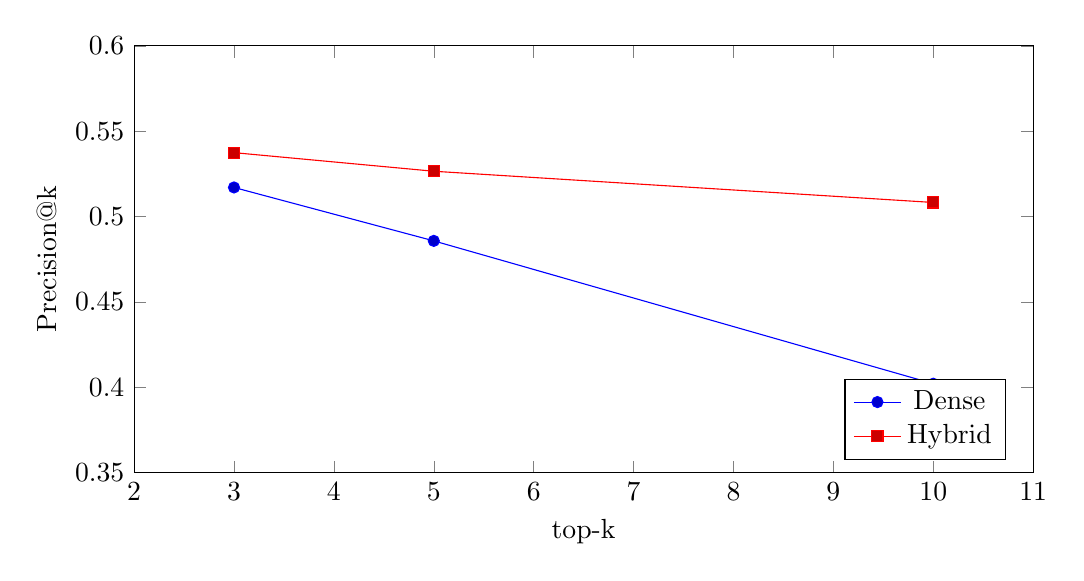
\begin{tikzpicture}
\begin{axis}[
width=13cm,
height=7cm,
xlabel={top-k},
ylabel={Precision@k},
xmin=2,xmax=11,
ymin=0.35,ymax=0.60,
legend pos=south east
]
\addplot coordinates {(3,0.5170)(5,0.4857)(10,0.4020)};
\addlegendentry{Dense}

\addplot coordinates {(3,0.5374)(5,0.5265)(10,0.5082)};
\addlegendentry{Hybrid}
\end{axis}
\end{tikzpicture}
\caption{Precision@k vs top-k for Dense and Hybrid retrieval (reranking disabled).}
\end{figure}

\begin{figure}[htbp]
\centering
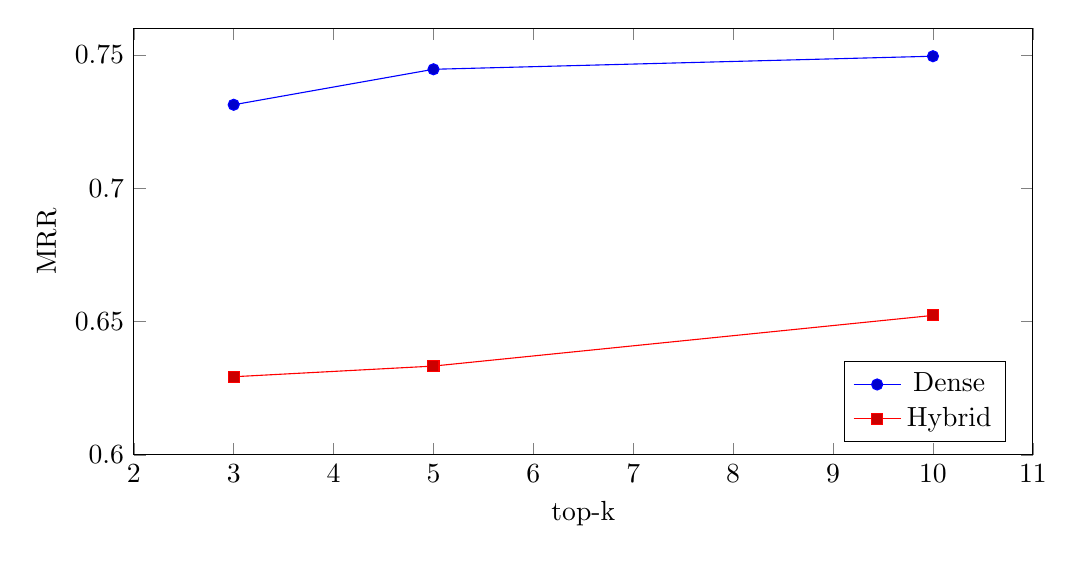
\begin{tikzpicture}
\begin{axis}[
width=13cm,
height=7cm,
xlabel={top-k},
ylabel={MRR},
xmin=2,xmax=11,
ymin=0.60,ymax=0.76,
legend pos=south east
]
\addplot coordinates {(3,0.7313)(5,0.7446)(10,0.7495)};
\addlegendentry{Dense}

\addplot coordinates {(3,0.6293)(5,0.6333)(10,0.6523)};
\addlegendentry{Hybrid}
\end{axis}
\end{tikzpicture}
\caption{MRR vs top-k for Dense and Hybrid retrieval (reranking disabled).}
\end{figure}

\newpage

\section{Discussion}

\subsection{Chunking as a Primary Design Variable}

The largest gains came from chunking rather than reranking or retrieval fusion. This suggests chunking should be treated as a core modeling decision rather than preprocessing.

Scientific papers contain uneven information density. Very small chunks lose context, while very large chunks dilute relevance. Fixed windows appear to offer a robust compromise.

\subsection{Dense vs Hybrid Retrieval}

Dense retrieval outperformed hybrid retrieval in this benchmark. Possible explanations include:

\begin{itemize}
    \item embeddings already captured most lexical relevance,
    \item BM25 weighting was not fully tuned,
    \item scientific terminology benefits more from semantic similarity than token overlap.
\end{itemize}

Dense retrieval methods have demonstrated strong semantic retrieval capabilities in open-domain retrieval settings \cite{karpukhin2020dpr}. However, this result should not be interpreted as universal superiority of dense retrieval, only that it was better aligned with the current corpus and benchmark.

\subsection{Reranking Trade-Offs}

Cross-encoder reranking improved Precision@k in some low-k settings but often reduced Recall@k. This makes reranking most useful when users need the highest-quality top few passages rather than broader evidence coverage.

\subsection{Retrieval Metrics vs Generation Quality}

Although Fixed Window Overlap achieved the best benchmark metrics, generation behavior may still differ across chunking strategies because larger chunks can preserve more discourse continuity.

This highlights an important limitation of retrieval-only benchmarks: better chunk-level metrics do not always guarantee better final responses. In this project, however, configuration selection was performed strictly with retrieval metrics and did not include generated-answer scoring.

\subsection{Recommended Evaluation Configuration}

For the current benchmark setup, the strongest retrieval-first configuration is:

\begin{itemize}
    \item Fixed Window Overlap
    \item Dense retrieval
    \item top-k = 10
    \item reranking disabled
\end{itemize}

Future systems may benefit from adaptive routing, where short factoid queries use small windows and explanatory queries use larger section-level evidence.

\newpage

\section{Limitations}

This project has several limitations:

\begin{itemize}
    \item only 49 benchmark queries were used,
    \item relevance judgments partly depended on similarity thresholds,
    \item only one embedding model family was tested,
    \item generation quality was not measured quantitatively,
    \item scientific domains differ substantially in terminology and structure.
\end{itemize}

Taken together, these limitations mean the reported results should be interpreted as strong evidence for this specific benchmark setup rather than as universally generalizable conclusions across all scientific RAG scenarios.

\section{Conclusion}

This report presented the practical implementation and optimization of ArxivRAG. Results showed that retrieval quality depends strongly on engineering choices rather than model scale alone.

Among four chunking methods, Fixed Window Overlap performed best quantitatively. Dense retrieval consistently exceeded hybrid retrieval, while reranking primarily functioned as a precision enhancement tool.

The strongest overall operating point achieved Recall@10 of 0.9592 and MRR of 0.7495. More broadly, the project demonstrates that effective scientific RAG systems require careful optimization of corpus construction, segmentation, indexing, and ranking.

The future objective of the project is to evolve ArxivRAG into a usable application with a lightweight UI, evidence transparency, configurability, and optimized generation.

\bibliography{references_practical}

\end{document}